\begin{figure}
    \begin{center}
    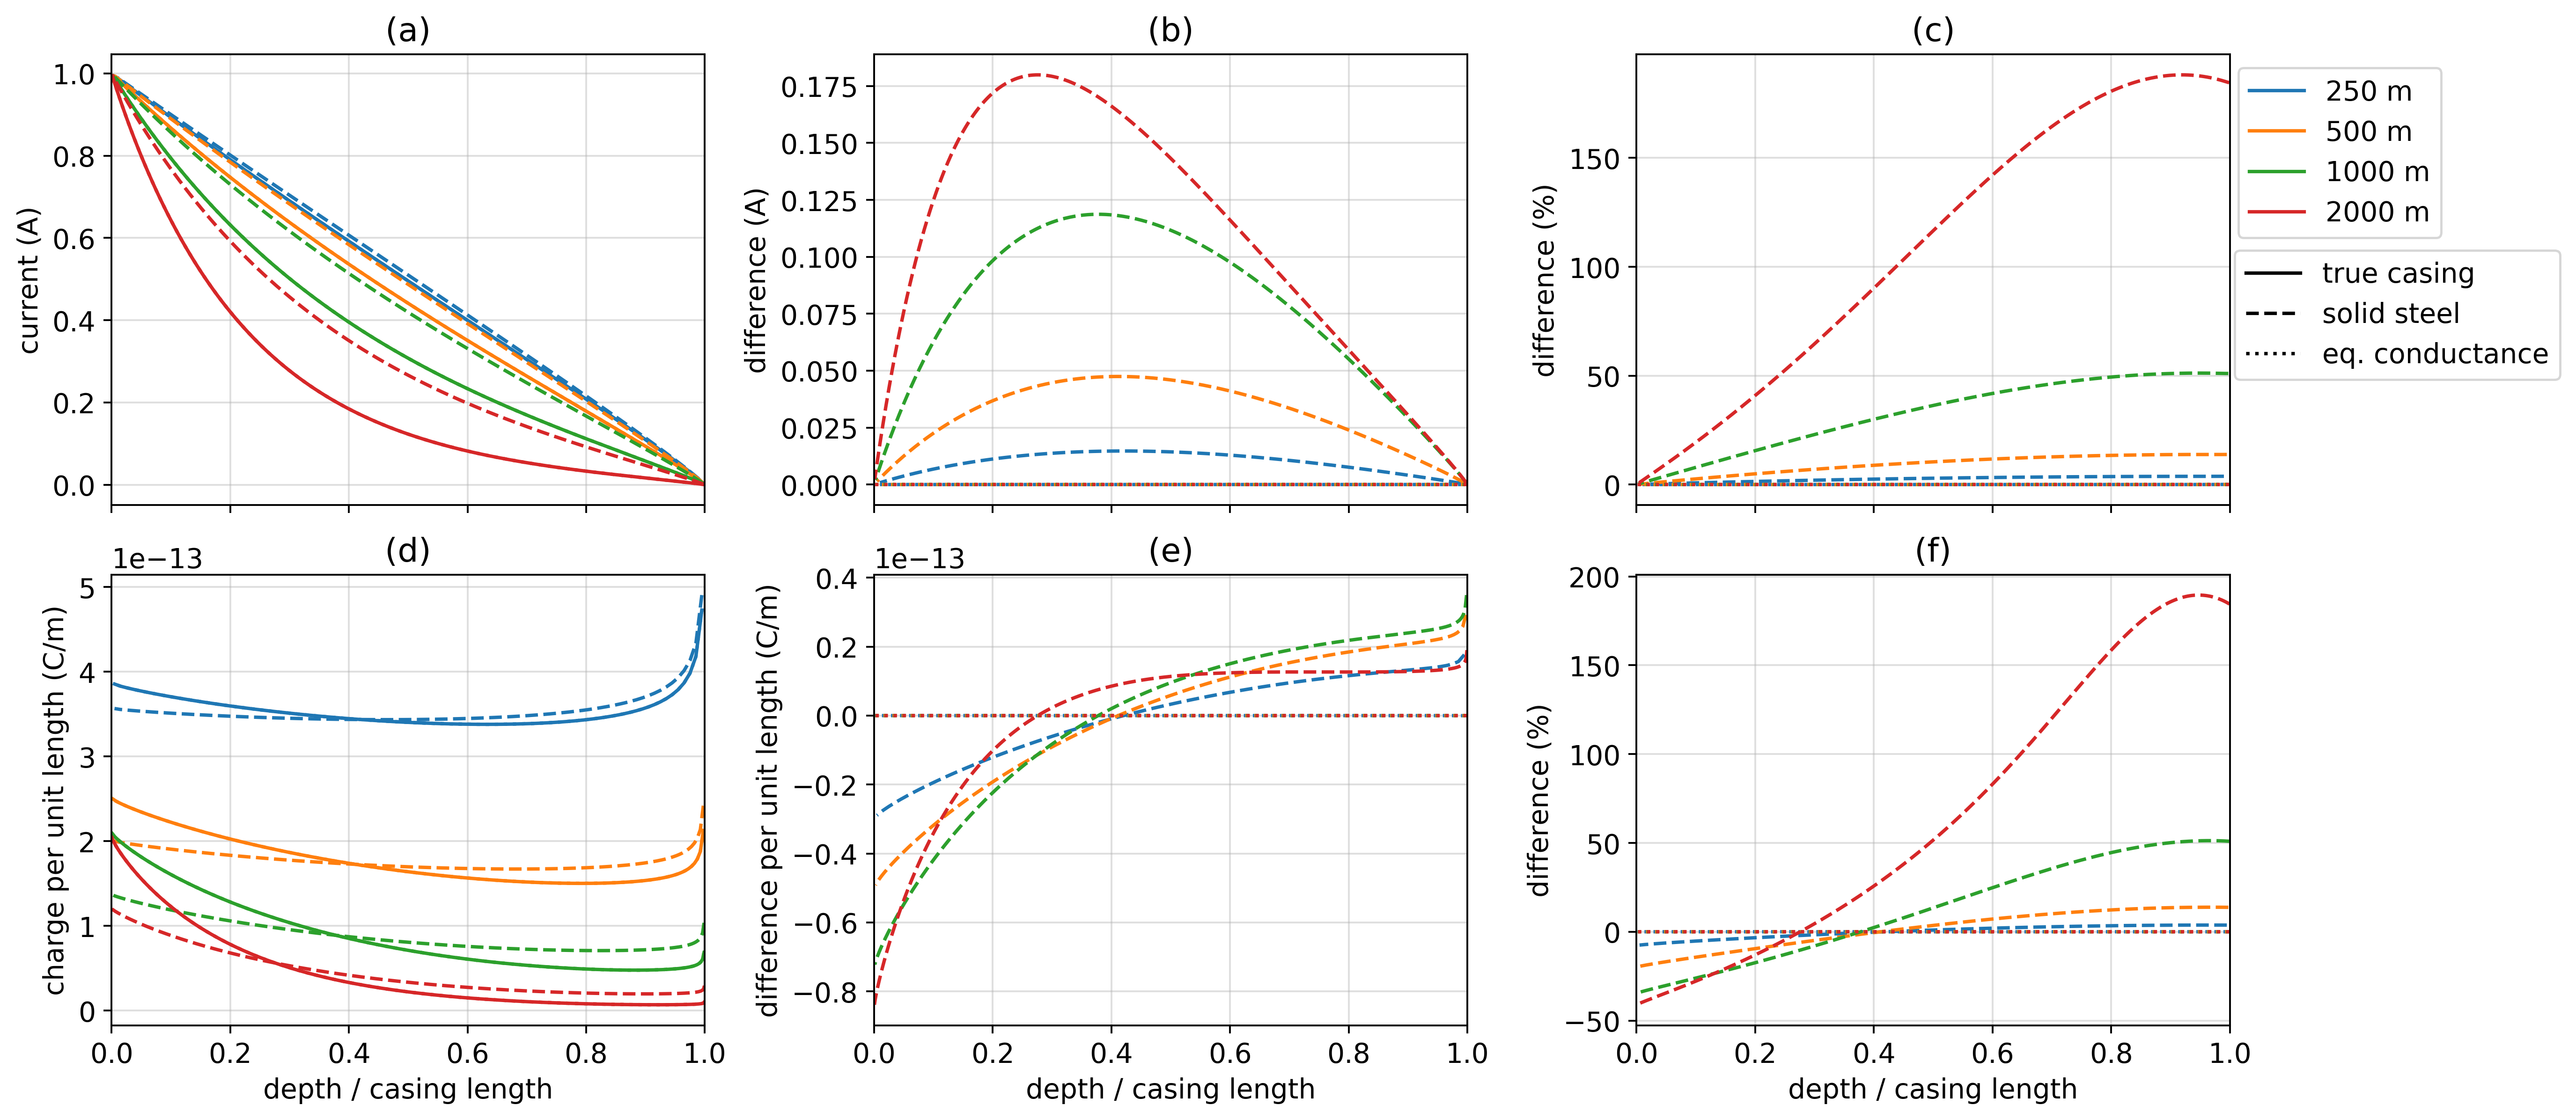
\includegraphics[width=\textwidth]{figures/approximating_wells_currents_charges.png}
    \end{center}
\caption{
    Currents (top row) and charges (bottom row) along the length of
    a hollow steel-cased well (solid lines), solid cylinder with
    conductivity equal to that of the steel-cased well (dashed-lines),
    and a solid cylinder with a conductivity such that the product of the
    conductivity and the cross sectional area of the cylinder is equal to that
    of the hollow-pipe (dotted lines). Each of the line-colors corresponds to a
    different casing length, as indicated in the legend.
    In (a), we show the vertical current in the casing,
    (b) shows the difference from the true, hollow-cased well
    in the vertical current within the casing, and (c) shows that difference as a percentage
    of the true currents. In (d), we show the charge per unit length along the casing, (e)
    shows the difference from the true, hollow-cased well and (e) shows that differences as
    a percentage of the true charge distribution.
    The x-axis on all plots is depth normalized by the length of the casing.
}
\label{fig:approximating_wells_currents_charges}
\end{figure}
